% 第四章 生成场景的质量验证
\chapter{生成场景的质量验证}
\section{实验设置}
\textbf{(1)测试数据集构成} \par
测试数据集是为了综合体现自动驾驶场景多样复杂特点,涵盖像直行障碍、转弯障碍等多种典型场景类别,例如直行障碍、转弯障碍、变道、超车、闯红灯、无保护左转、右转以及交叉路口协商等,这些场景类别覆盖自动驾驶车辆实际道路环境可能遇到的关键交互情况,具备较高代表性和实用价值。数据集中场景描述以自然语言形式进行呈现,并且包含一定比例模糊性描述,以此模拟真实世界里驾驶员或其他交通参与者行为不可预测性,场景描述模糊性设计有助于测试生成系统应对不精确指令时的处理能力,确保系统能够适应并生成符合要求的复杂交通场景。\\
\indent\textbf{(2)对比基线选择依据} \par
在评估生成场景的质量的时候本研究选用两种有代表性方法作基线对比,基于规则的方法也就是Rule - based这种方法通过定义明确逻辑和规则来生成场景具有较好可解释性适合处理结构化和预定义任务,不过在面对复杂和模糊的自然语言描述时其灵活性和适应性比较差。
基于GPT - 4.0的方法是借助大型语言模型生成能力,以此生成丰富多样的场景,该方法在场景生成多样性方面具备优势,不过在生成场景的物理合规性和逻辑一致性上存在不足,特别是在处理复杂交通情境的时候。
选择这两种基线的主要目的是从不同角度评估本研究方法在生成场景质量、效率以及针对复杂和模糊指令的鲁棒性方面所具备的优势。\\
\indent\textbf{(3)硬件平台与评估指标} \par
硬件平台:本实验使用联想Y900P高性能笔记本电脑。该平台配置了多核的 Intel Core i9 处理器可以高效处理复杂的计算任务,以此确保场景生成实时性与响应速度,此外配备的专业级显卡,能为图形处理和并行计算任务提供强大支持,特别是在大规模场景生成过程中,系统还配备大容量内存和高速固态硬盘(SSD),保证数据处理和存储工作高效且稳定。

评估指标方面,为全面评估生成场景的质量本研究采用以下几个关键指标,场景生成时间指标,它衡量生成一个场景所需的时间能反映系统的效率,较短生成时间有助于提高测试灵活性和响应速度,场景物理合规性方面,评估生成场景是否符合物理约束条件如车辆最大加速度和最小转弯半径等,物理合规性能确保场景真实性使生成场景能反映自动驾驶系统实际驾驶条件。


检查场景中各元素之间逻辑关系是否合理确保生成场景符合法定交通规则这是场景逻辑一致性的要求逻辑一致性是验证场景真实性和可接受性的核心标准,统计生成场景的类型和数量以此衡量系统的多样性和生成能力多样性高的系统可为自动驾驶系统提供更广泛测试场景进而有效覆盖更多潜在驾驶情况这是场景多样性的体现,在仿真环境中运行生成的场景并统计发生碰撞的频率碰撞率反映生成场景的安全性较低碰撞率意味着生成场景能较好模拟真实世界的安全驾驶环境。




\section{生成效果展示(示例)}

\subsection{场景一:摩托车和汽车在红绿灯前等待信号}
\indent 一辆摩托车和一辆汽车在红绿灯前等待信号。\\

\begin{figure}[H]
	\centering
	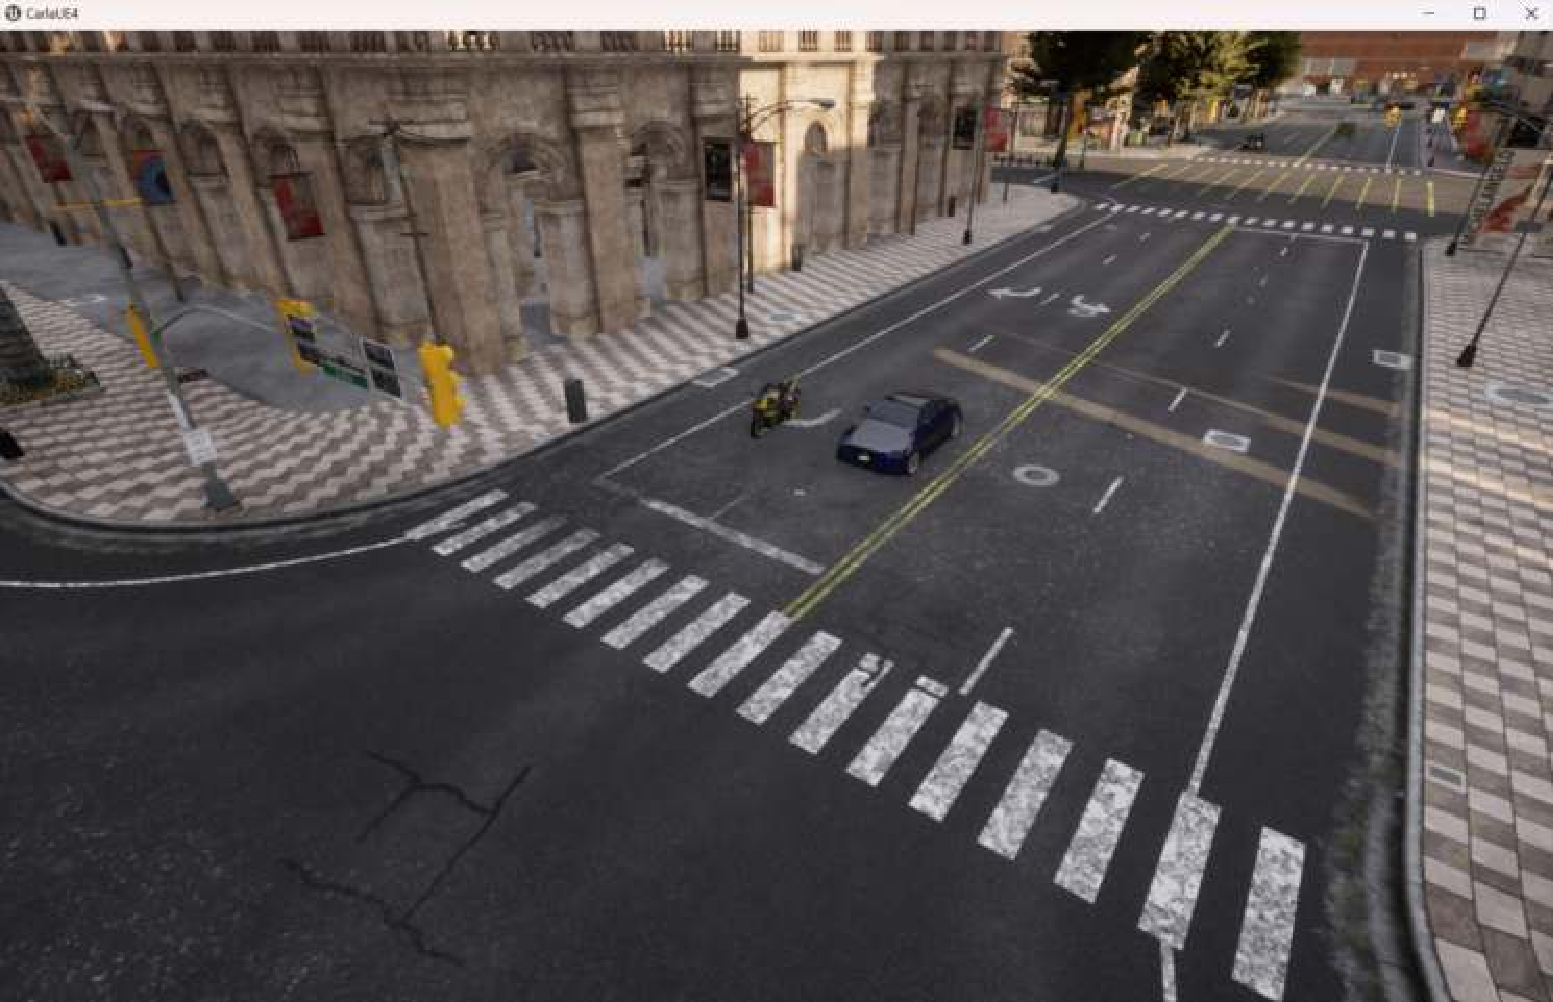
\includegraphics[width=1.0\textwidth]{"images/1.pdf"}
	\caption{摩托车与汽车在红绿灯前等待信号的场景截图}
	\label{fig:redlight_motorbike_car}
\end{figure}

\subsection{场景二:自我车辆在夜晚穿越道路}
\indent 在夜晚,一些自我车辆正在穿越道路,街道上的路灯微弱地照亮着周围环境,远处偶尔可以看到其他车辆的车灯闪烁。\\

\begin{figure}[H]
	\centering
	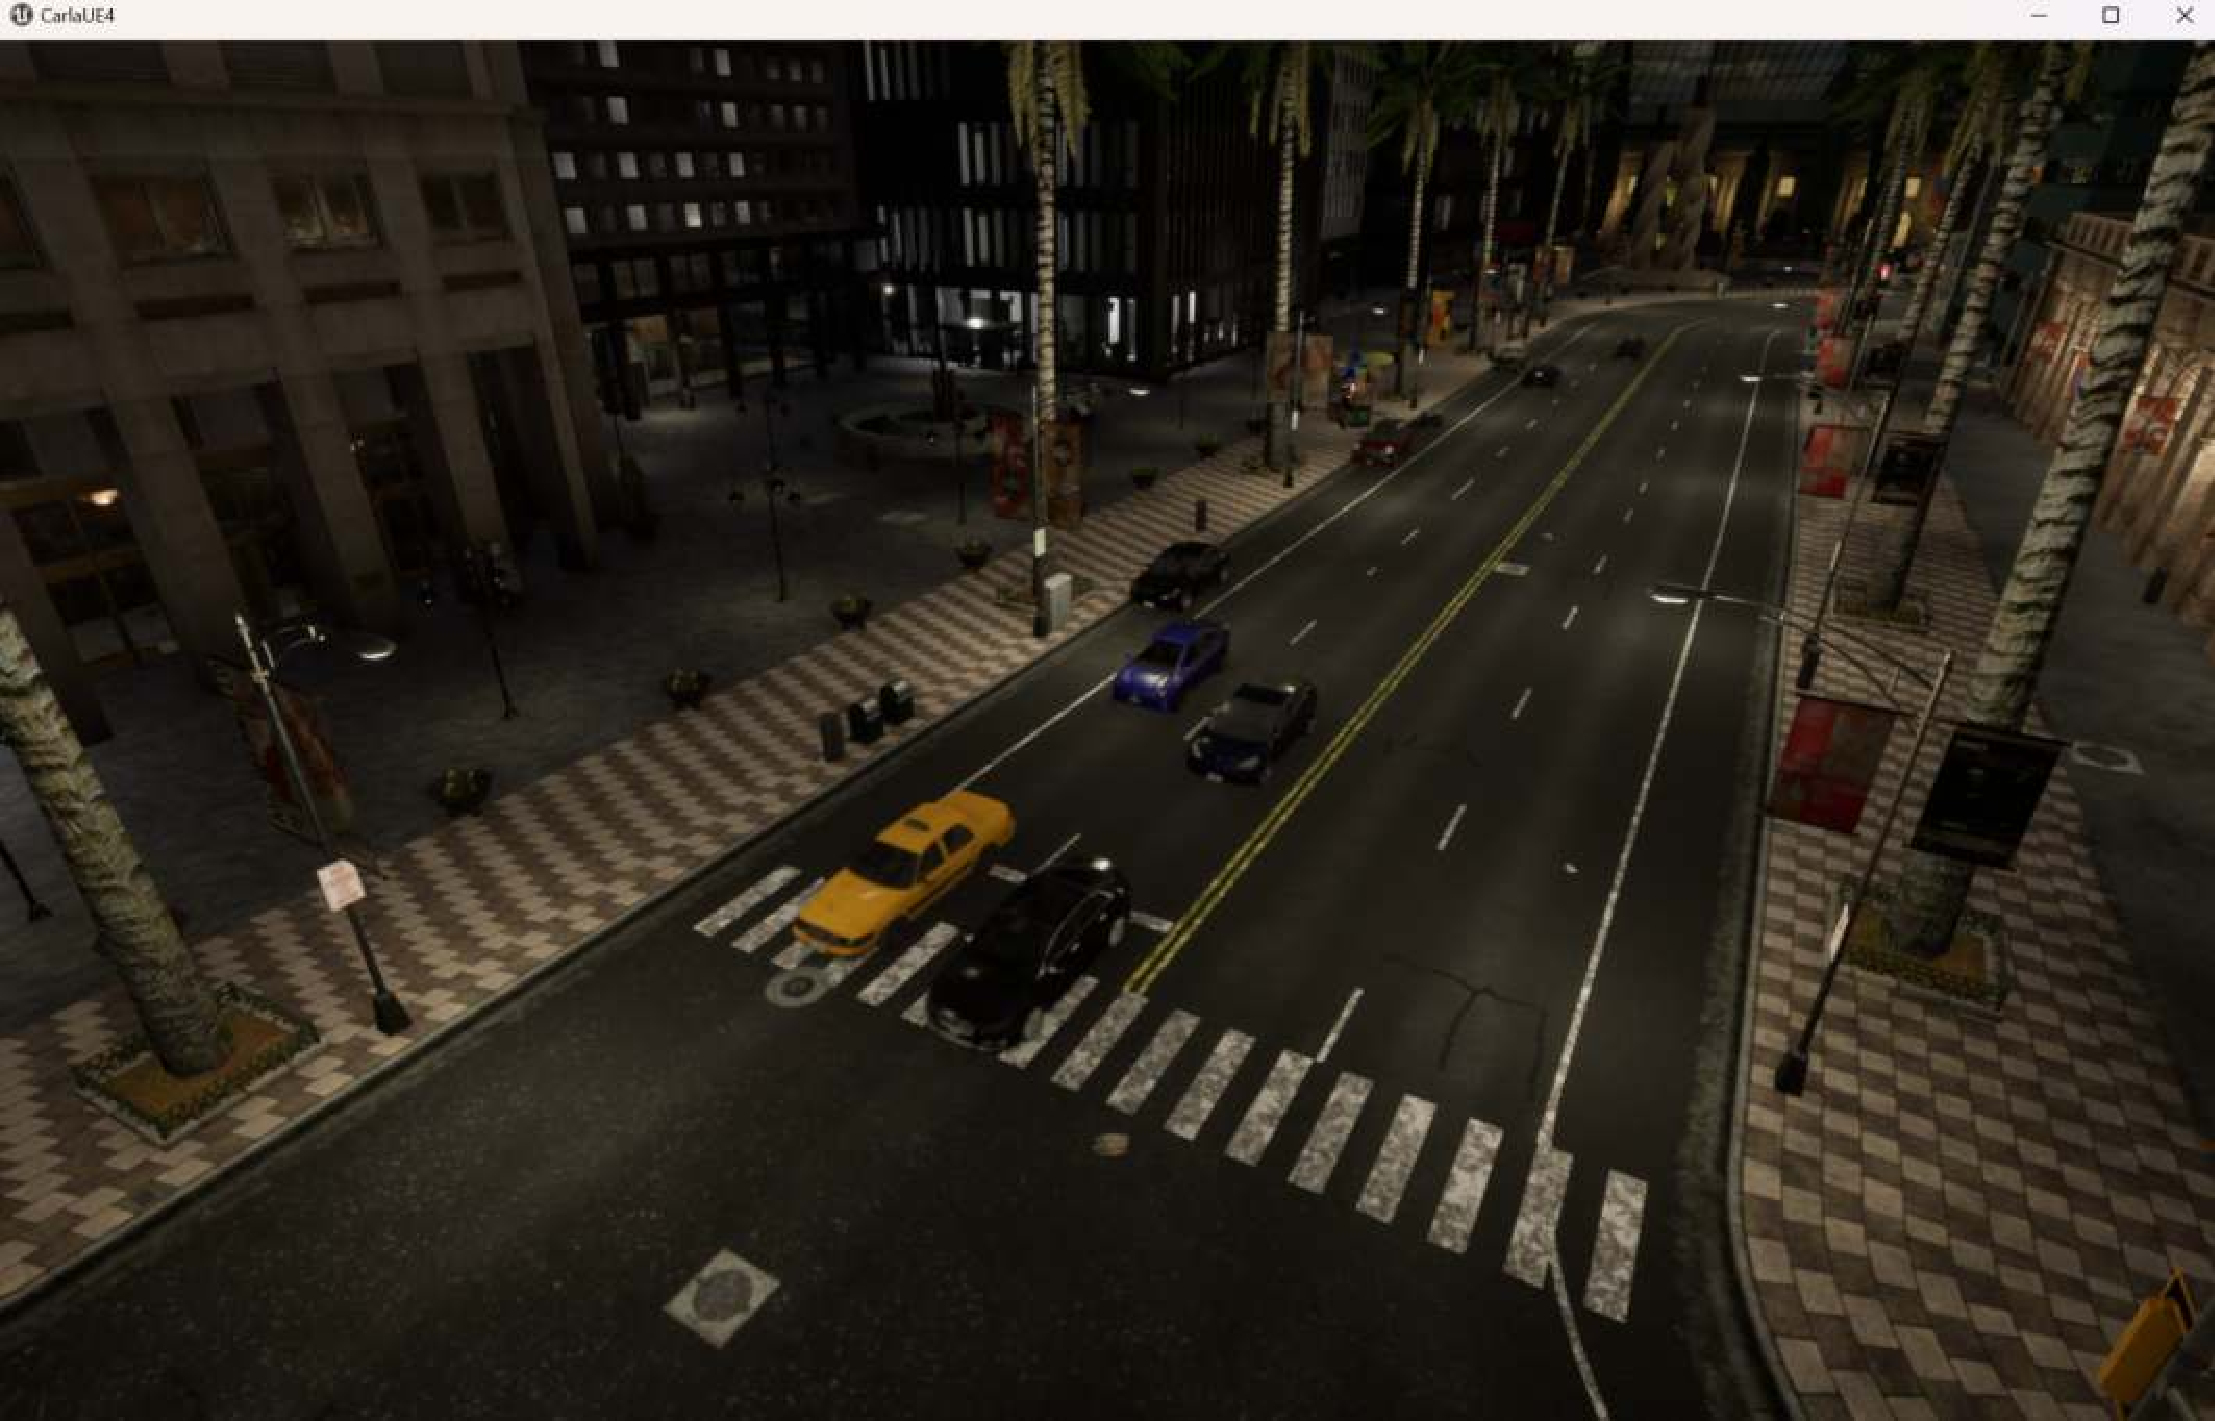
\includegraphics[width=1.0\textwidth]{"images/2.pdf"}
	\caption{自我车辆在夜晚穿越道路的场景截图}
	\label{fig:night_self_driving_cross}
\end{figure}

\subsection{场景三:自我车辆在夜晚红绿灯前等待信号}
\indent 在夜晚,一些自我车辆在红绿灯前等待信号,而在另一方向,自我车辆正在通行,车灯的光芒穿过昏暗的街道。\\

\begin{figure}[H]
	\centering
	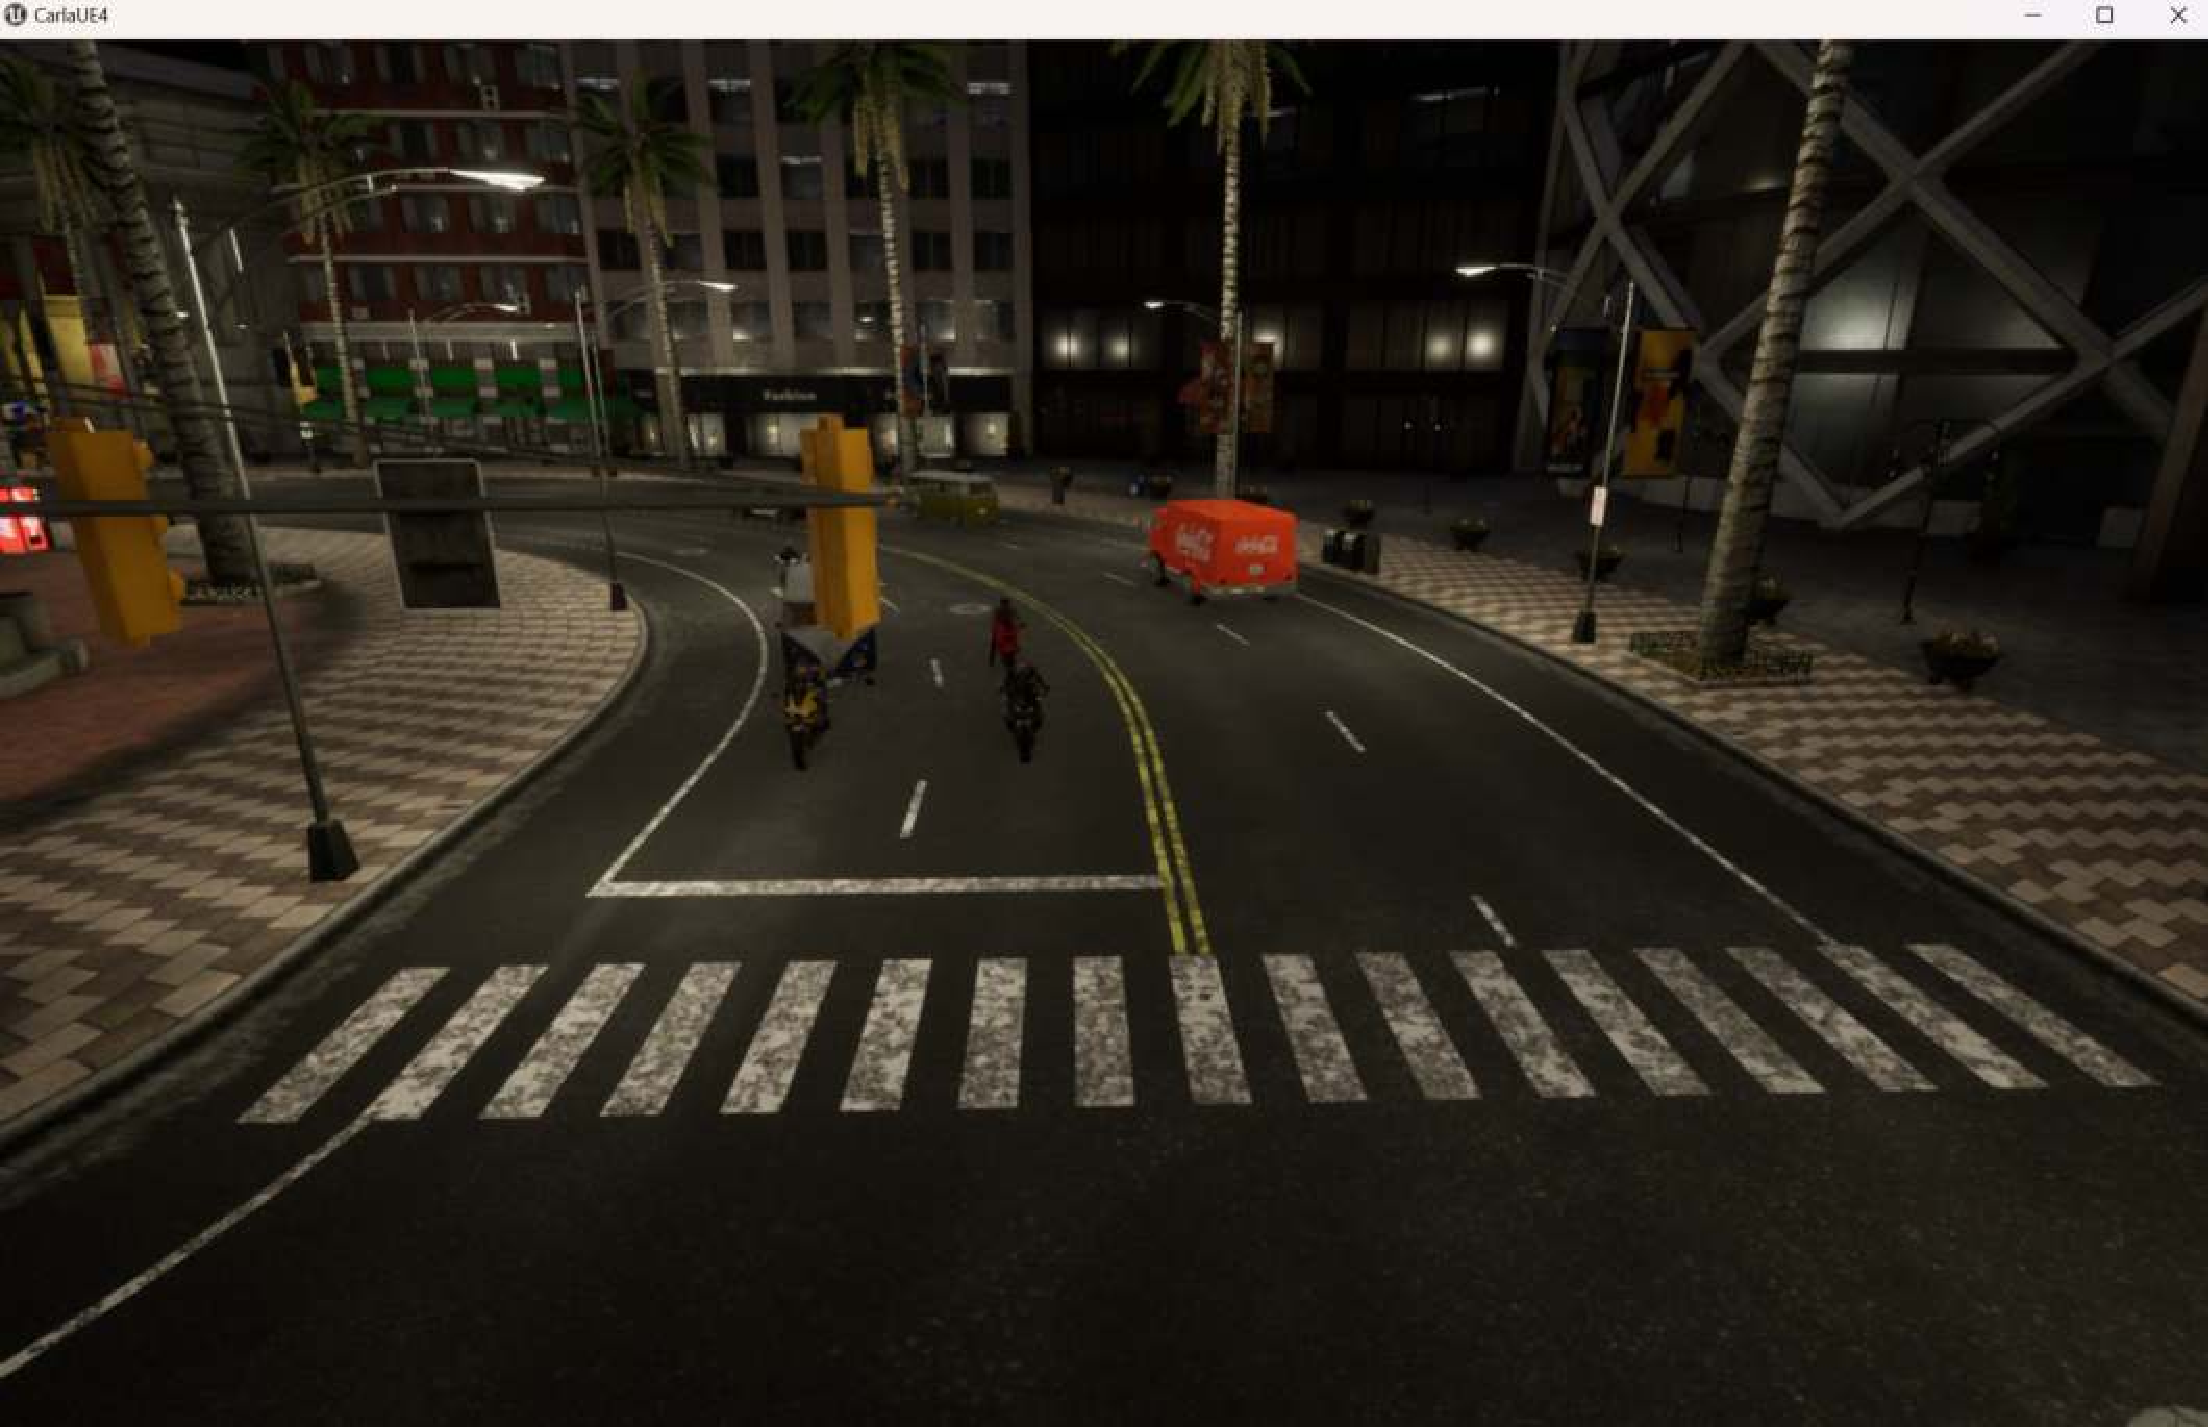
\includegraphics[width=1.0\textwidth]{"images/4.pdf"}
	\caption{自我车辆在夜晚红绿灯前等待信号的场景截图}
	\label{fig:night_redlight_cross}
\end{figure}

\subsection{场景四:行人横穿直行道路}
\indent 自我车辆在笔直的道路上行驶时,一名行人突然从右前方横穿过来,并在自我车辆接近时突然停下。\\

\begin{figure}[H]
	\centering
	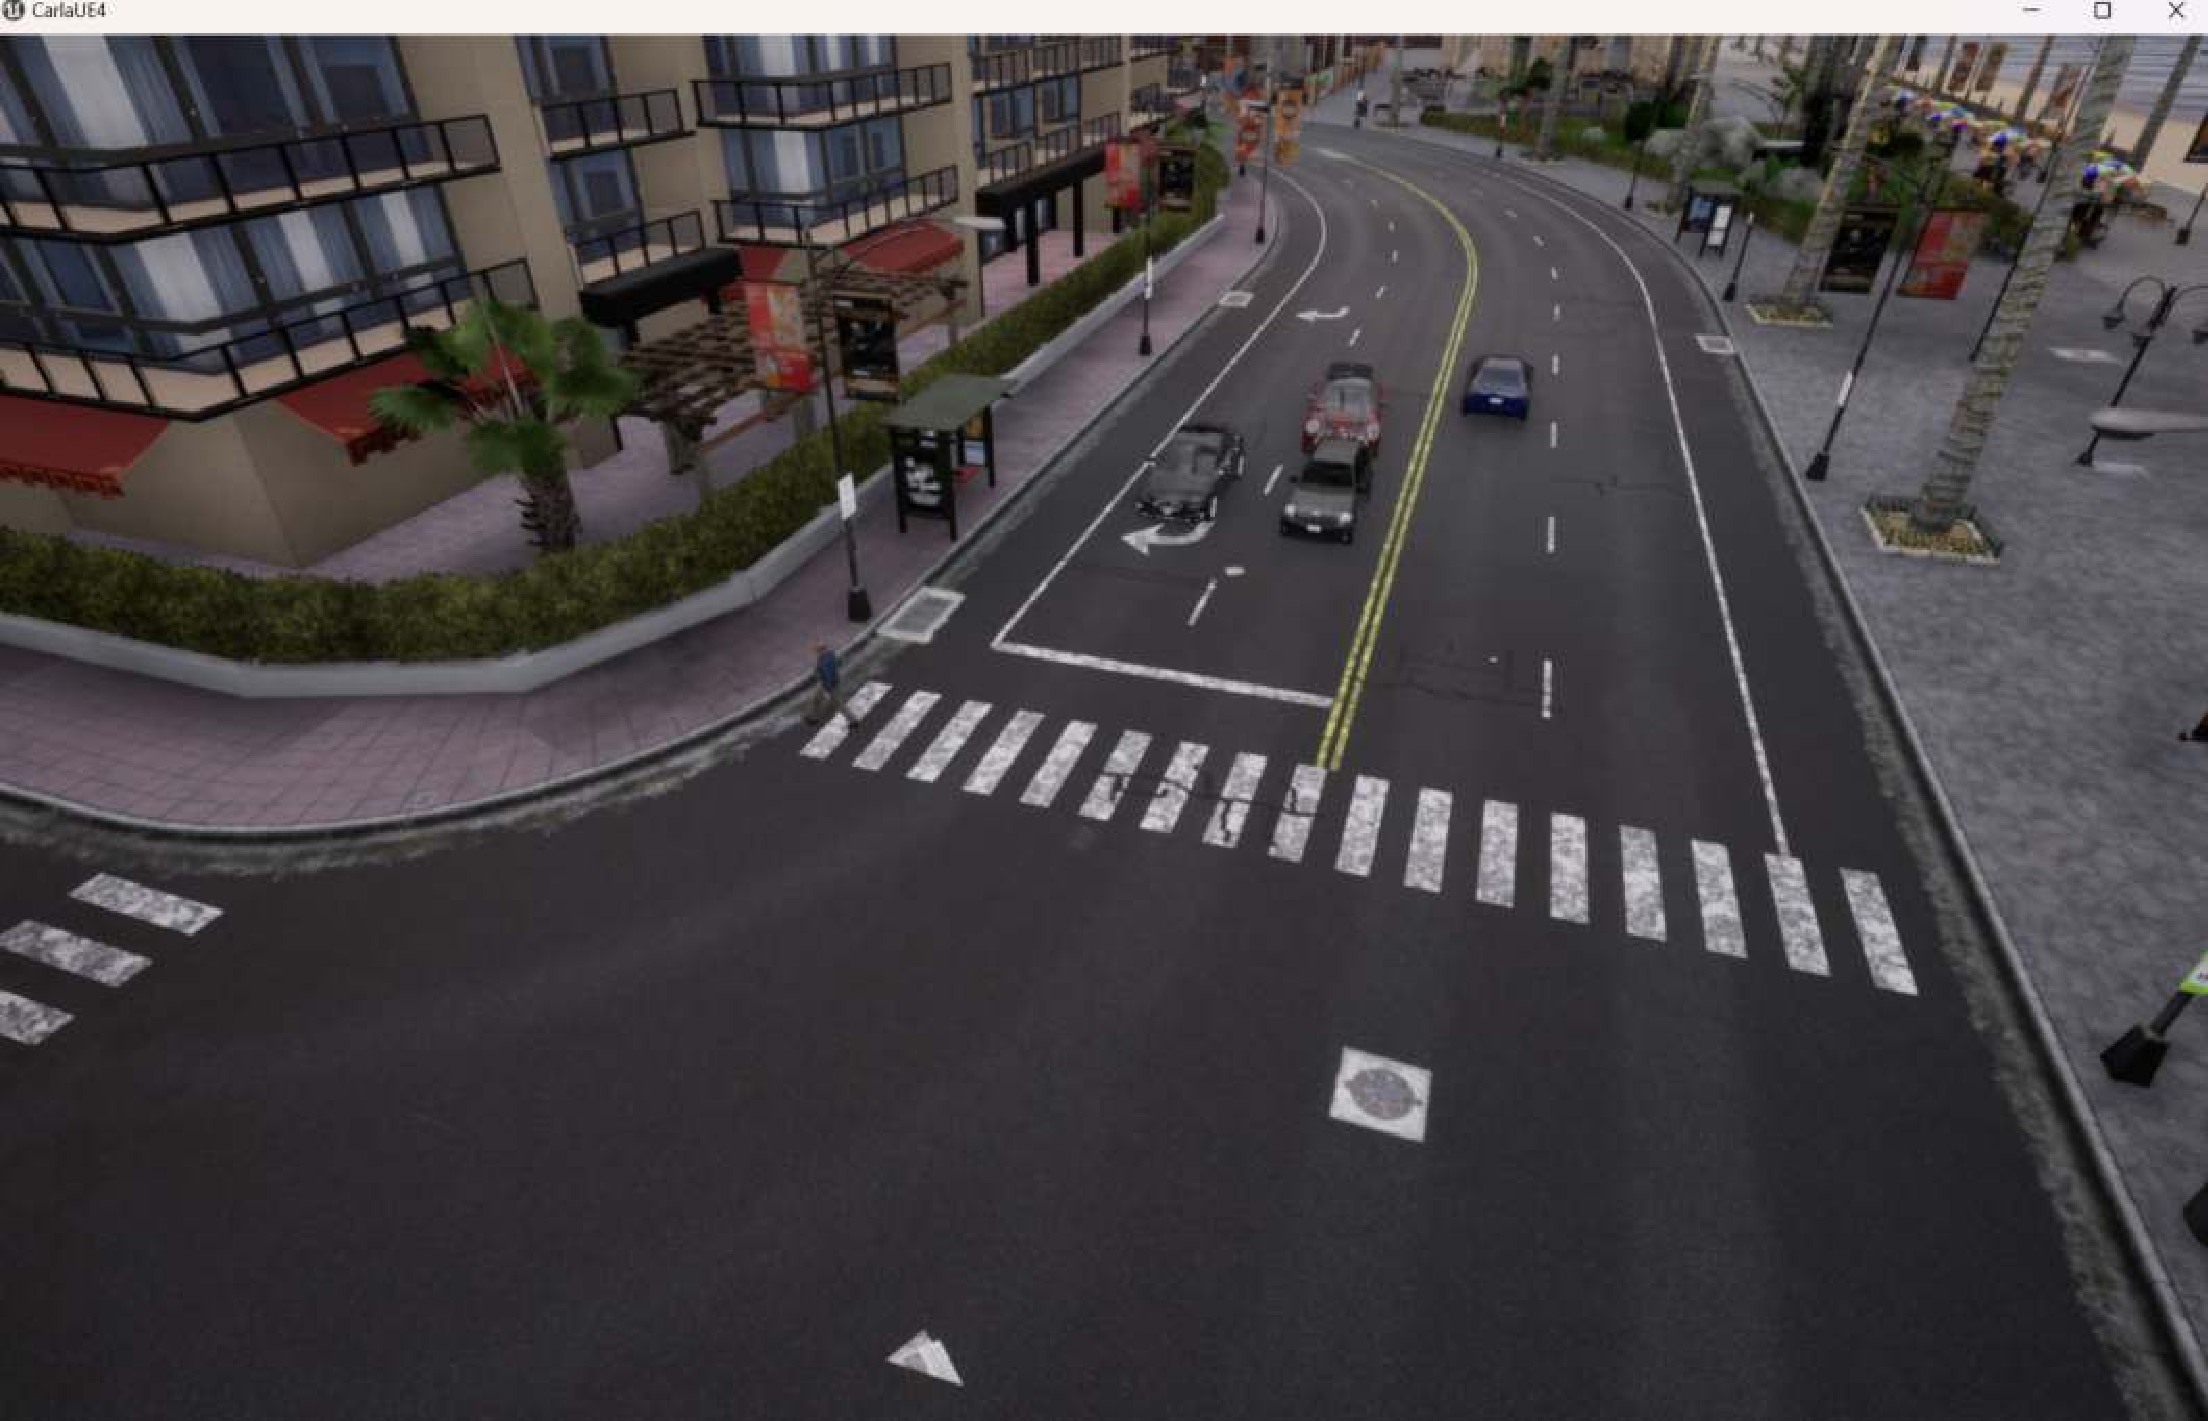
\includegraphics[width=1.0\textwidth]{"images/5.pdf"}
	\caption{行人横穿直行道路的场景截图}
	\label{fig:pedestrian_crossing}
\end{figure}
\subsection {更多}
\begin{figure}[H]
	\centering
	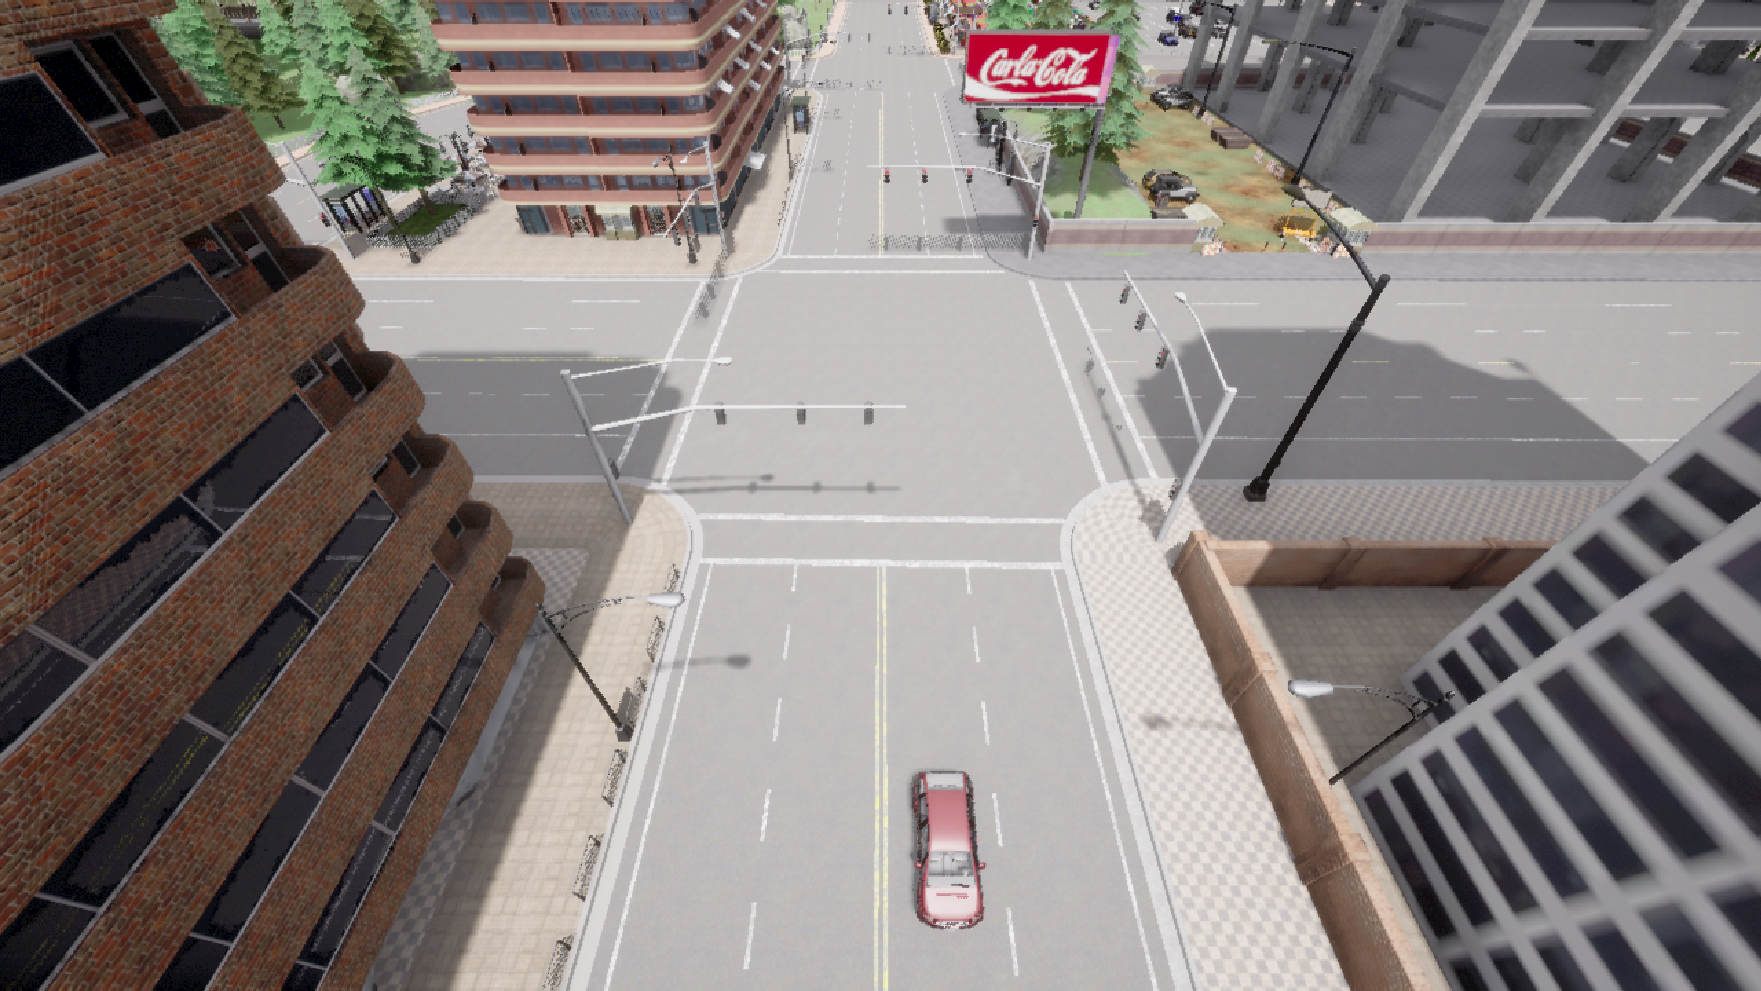
\includegraphics[width=1.0\textwidth]{"images/场景5.pdf"}
	\caption{场景截图}
	\label{}
\end{figure}
\begin{figure}[H]
	\centering
	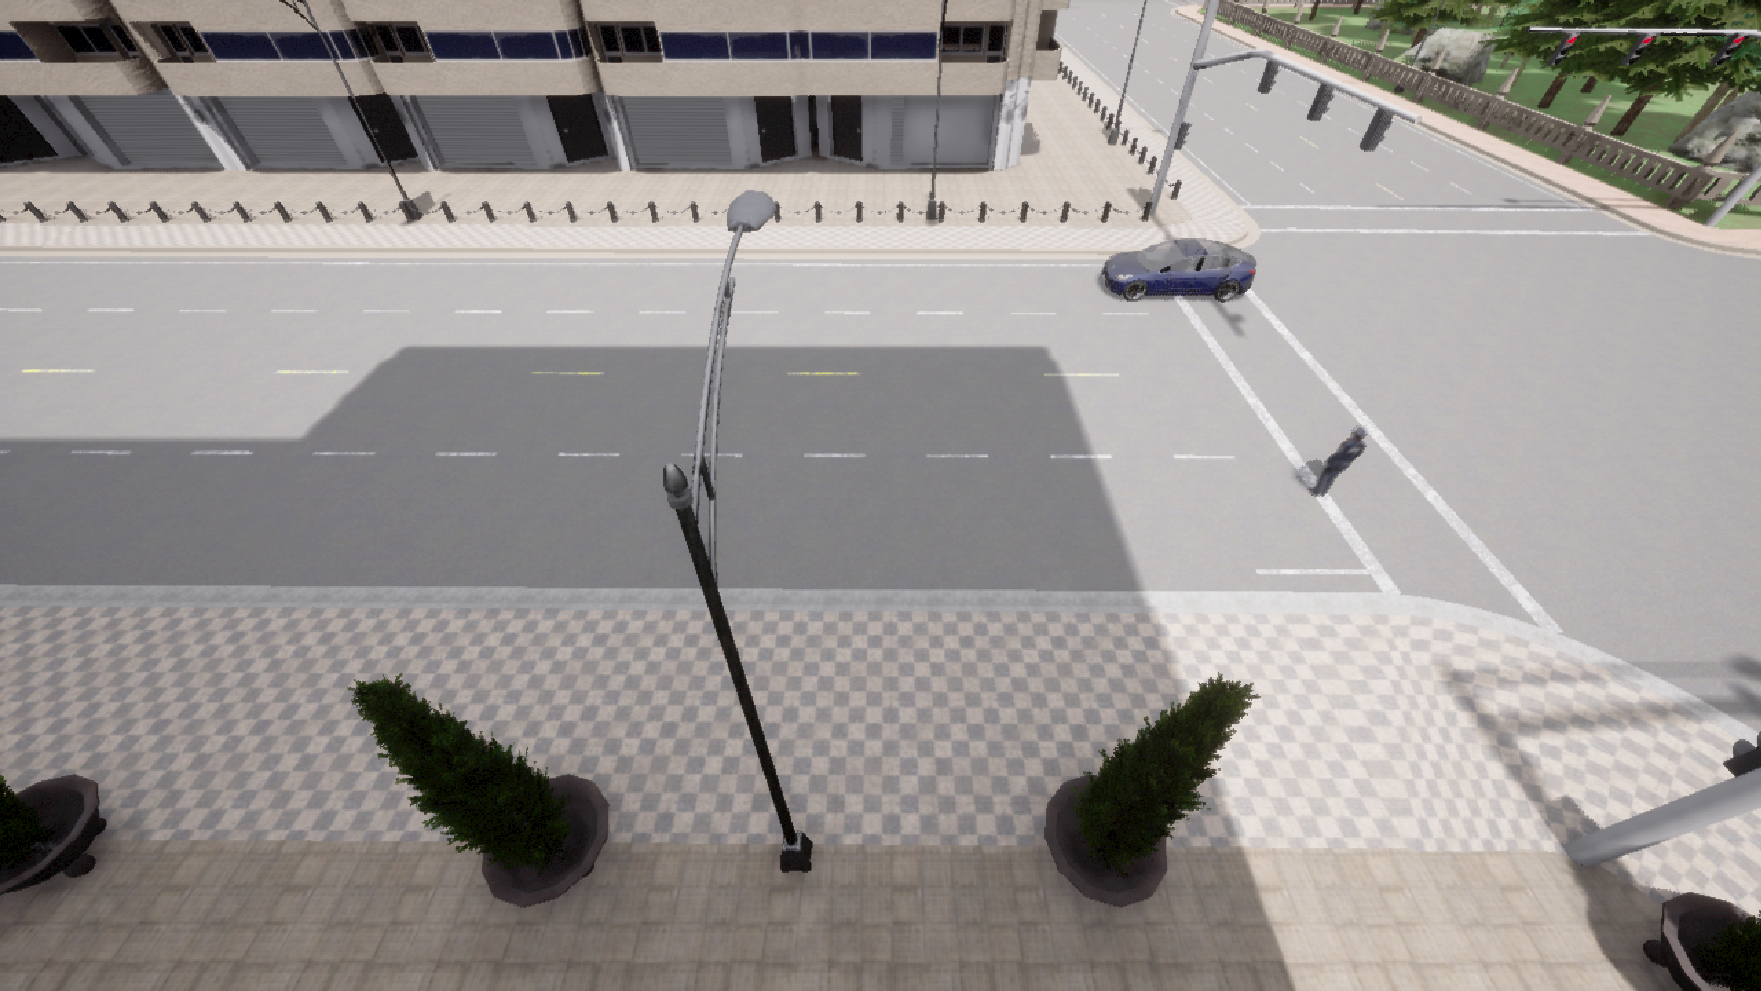
\includegraphics[width=1.0\textwidth]{"images/场景6.pdf"}
	\caption{场景截图}
	\label{}
\end{figure}
\begin{figure}[H]
	\centering
	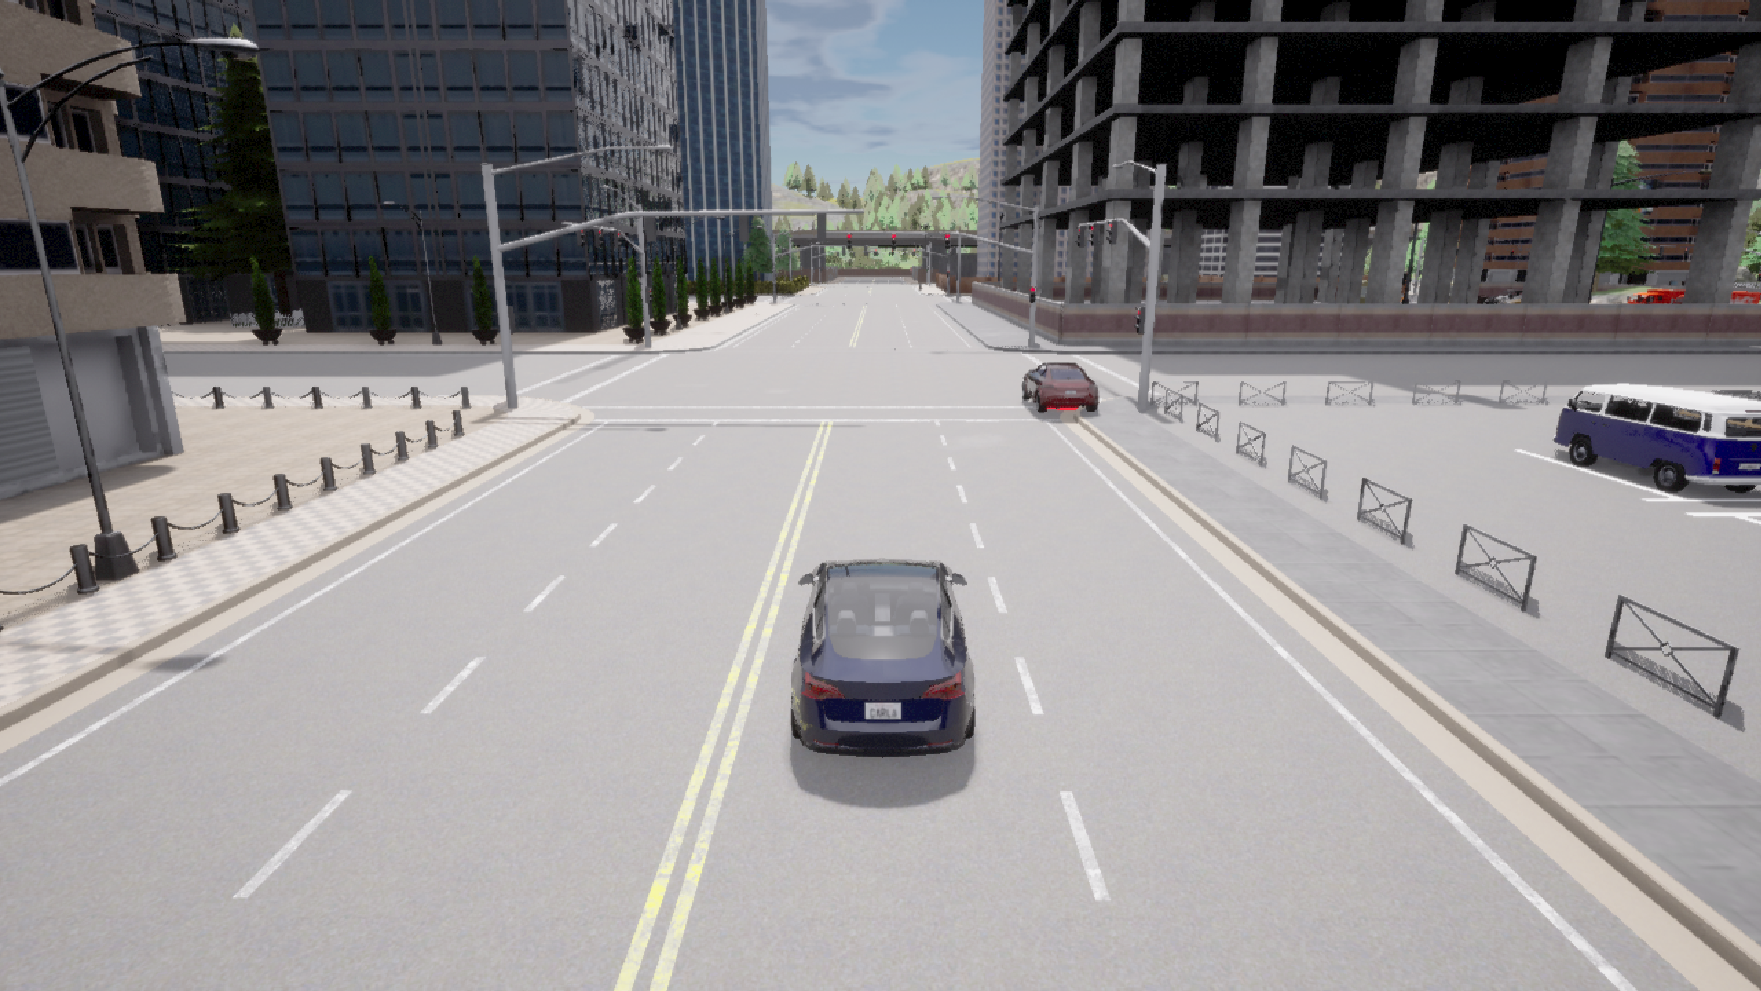
\includegraphics[width=1.0\textwidth]{"images/场景7.pdf"}
	\caption{场景截图}
	\label{}
\end{figure}
\begin{figure}[H]
	\centering
	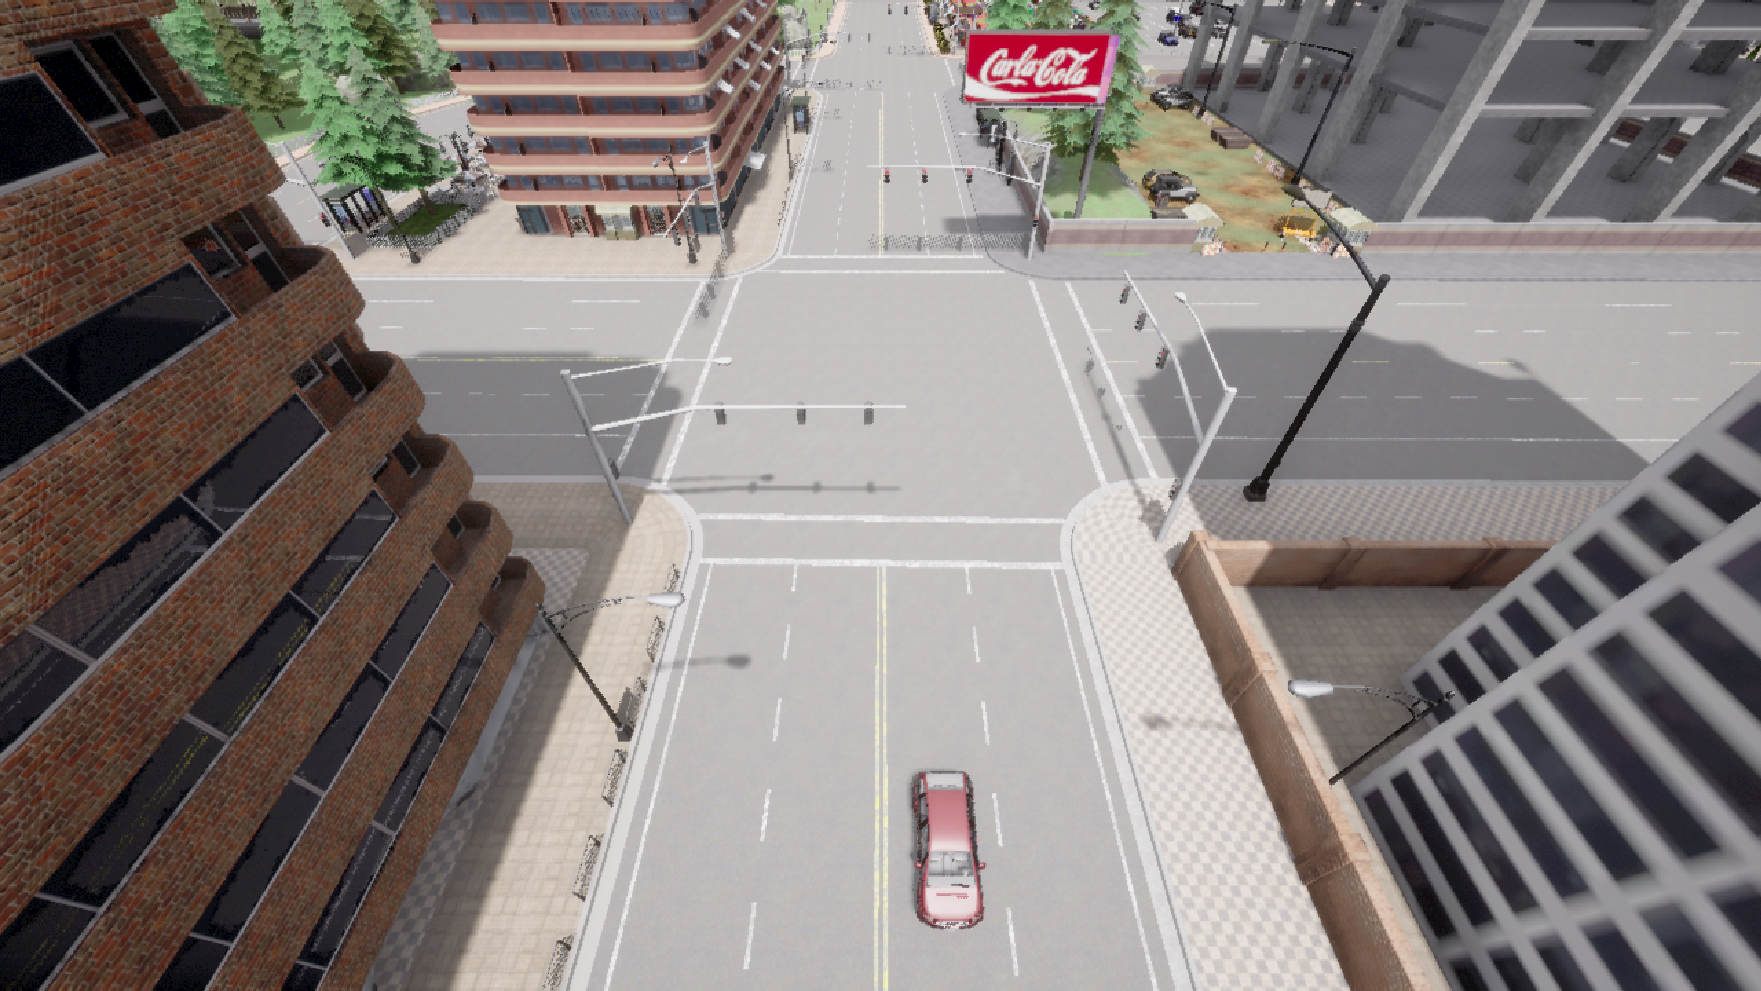
\includegraphics[width=1.0\textwidth]{"images/场景8.pdf"}
	\caption{场景截图}
	\label{}
\end{figure}
\begin{figure}[H]
	\centering
	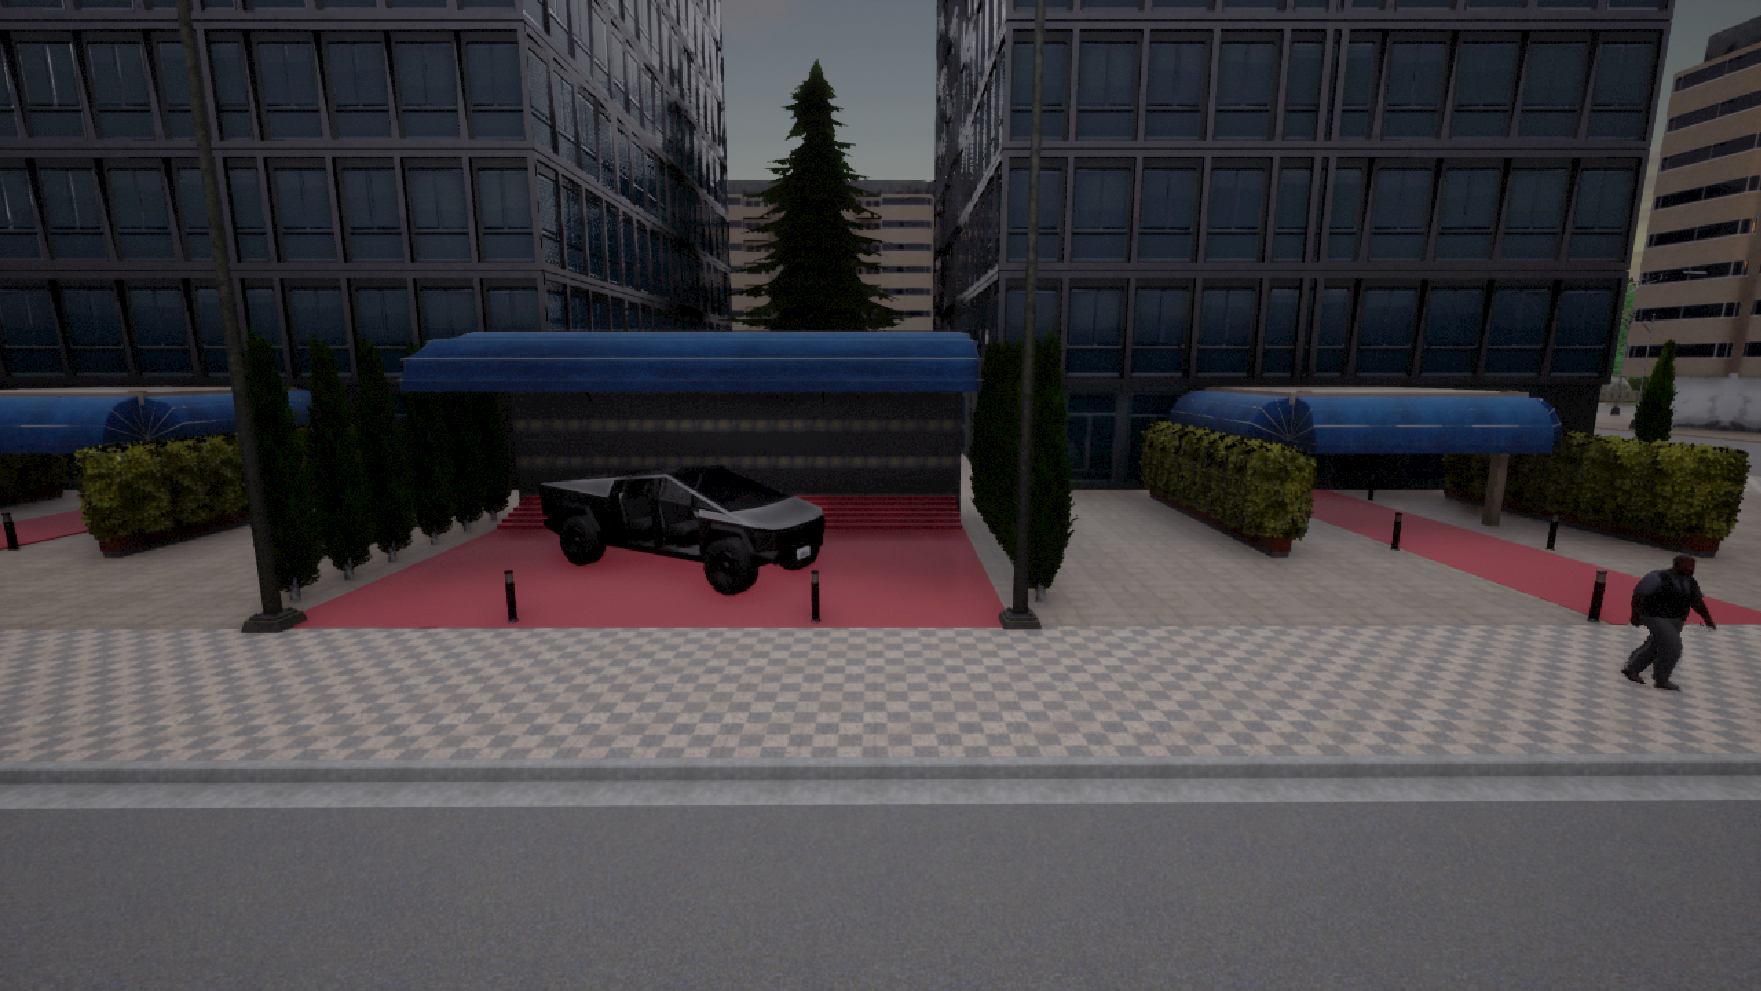
\includegraphics[width=1.0\textwidth]{"images/场景9.pdf"}
	\caption{场景截图}
	\label{}
\end{figure}
\begin{figure}[H]
	\centering
	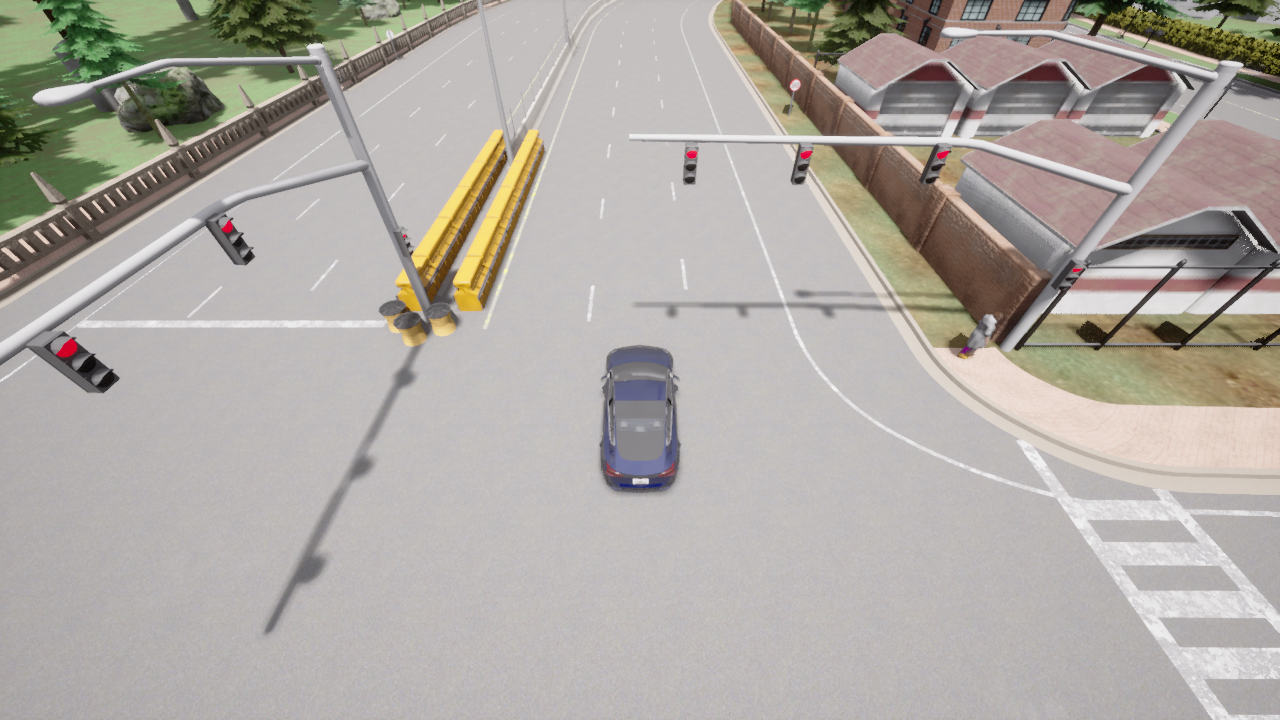
\includegraphics[width=1.0\textwidth]{"images/场景10.pdf"}
	\caption{场景截图}
	\label{}
\end{figure}
\section{实验总结}

这一章主要描述的是基于自然语言生成三维交通场景的核心流程,也就是“语言描述 → 场景代码生成 → 仿真构建”,这个流程展示了借助自然语言输入、自动脚本生成以及仿真执行的技术路径,来实现复杂三维交通场景高效构建的方式。

\begin{itemize}
	\item \textbf{自然语言解析}\texttt{scenario\_descriptions.txt}文件获取自然语言描述,每条描述都代表着一个特定的交通场景,涵盖交通参与者类型数量初始位置及行为意图等信息,用户通过直观的语言输入来定义所需的场景特征,系统借助\texttt{retrieve.py}脚本对输入的自然语言做语义解析,解析目标是从文本当中识别出场景的关键元素,例如车辆的种类行驶方向速度甚至动态行为,像超车停车避让等情况,该步骤主要依靠自然语言处理(NLP)技术,通过文本特征提取与词汇映射把模糊语言信息转为有结构的场景要素。
	
	\item \textbf{生成场景代码},系统就会按照预设规则与模板生成符合Scenic语法规范的场景脚本,Scenic是专门针对三维仿真场景描述的一种语言,其具有灵活且适用于动态场景建模的特点,系统依据输入描述所生成的代码涵盖场景中参与者的初始化设置,像车辆的位置、速度、运动轨迹等内容,还有可能存在的动态行为,例如交通参与者的交互、变道、超车等情况,生成的Scenic脚本具备可执行性,并且能够作为输入文件传递给Scenic编译器,此阶段自动化程度较高,在大部分场景下都能自动生成相应的场景代码,进而减少了人工干预的需求。
	
	\item \textbf{仿真场景构建与执行},生成的Scenic场景脚本会被传至仿真平台,主要就是CARLA,通过Scenic - CARLA接口来执行,CARLA是个开源的自动驾驶仿真平台,它能够依据场景脚本里的设置构建出真实感强且动态可控的三维仿真场景,在此过程当中,系统会按照Scenic脚本里的配置去加载地图、部署交通参与者像汽车行人等、设置场景初始状态比如天气时间环境条件等,仿真平台还会根据脚本里的动态行为设定实时执行参与者的运动轨迹与交互,举个例子,当脚本指定一辆车在道路上缓慢行驶并让行时,CARLA仿真平台会根据脚本设置准确模拟该行为,保证生成的仿真场景在空间和行为上都符合预期。
	
	\item \textbf{系统流程特性},“语言描述 → 场景代码生成 → 仿真构建”整个流程体现系统自动化处理能力,特别是自然语言到仿真场景代码生成的桥接,借助 \texttt{retrieve.py} 脚本,用户能通过文本输入快速生成三维交通场景,减少手动构建仿真场景的工作量,并且该流程支持生成复杂场景和动态交互行为,可精准还原交通系统中追尾、避让、变道等各种交互情境,为自动驾驶系统测试与评估提供有效支持。
	
\end{itemize}
\begin{figure}[H]
	\centering
	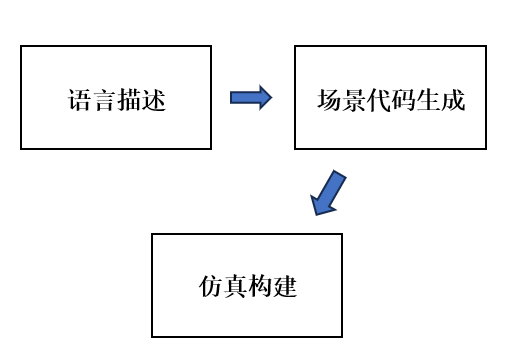
\includegraphics[width=1.0\textwidth]{"images/流程图1.pdf"}
	\caption{从自然语言描述到仿真场景构建的流程图}
	\label{fig:flowchart}
\end{figure}